%!TEX TS-program = pdflatex
%!TEX root = ../main.tex
%!TEX encoding = UTF-8 Unicode


\section[Conclusions]{Conclusions}
	
	\begin{frame}{Project workflow}
		\begin{figure}
			\centering
			\begin{tikzpicture}
   				\node[anchor=south west,inner sep=0] at (0,0) {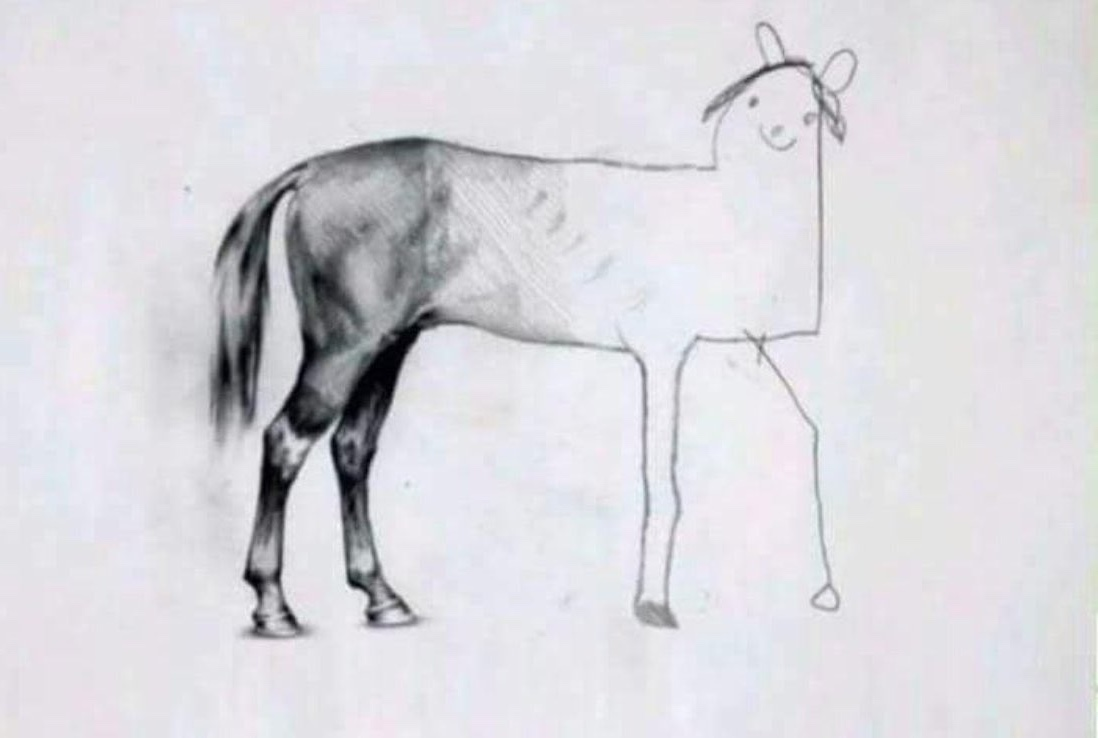
\includegraphics[width=.6\textwidth]{./images/horse.jpg}};
				
				\node[draw,align=center,fill=white,inner sep=1pt,font = {\scriptsize}] at (1.75,.2) {First\\month};
    	
				\draw[thick] (3.25,0) -- (3.25,5.65);

				\node[draw,align=center,fill=white,inner sep=1pt,font = {\scriptsize}] at (3.8,.2) {Second\\month};
    		
				\draw[thick] (4.35,0) -- (4.35,5.65);

				\node[draw,align=center,fill=white,inner sep=1pt,font = {\scriptsize}] at (4.9,.2) {Third\\month};

    			\draw[thick] (5.5,0) -- (5.5,5.65);
			
				\node[draw,align=center,fill=white,inner sep=1pt,font = {\scriptsize}] at (7,.2) {One week\\to the exam};

			\end{tikzpicture}

			\caption{The roadmap of our journey.}
			\label{fig:roadmap}
		\end{figure}
	\end{frame}
	
	\begin{frame}[allowframebreaks]{Lessons learned}
	We learned many things from this project:
	\begin{enumerate}
		\item not all papers found in the literature meet the necessary requirements for replicability;
	\end{enumerate}
	
	\framebreak
	
	And, most important, we learned that\dots
		
	\begin{quote}
    	It's all about the journey, not the destination.
    \end{quote}
	Thank you for your attention.
     
	\end{frame}